
\begin{questions}
\question{
Numerical solution
}
\begin{solution}
  In order to simplify my calculations I'm going to set my periodic potential as follows
  \begin{equation}
    U(x) = A\sum_{s}\delta(x-sa),\qquad s\in \mathbb{Z}
  \end{equation}
  where A is a constant and $a$ is the lattice parameter. We approximate this potential by spiked functions as we can see in fig. \ref{fig:delt}

  \begin{center}
    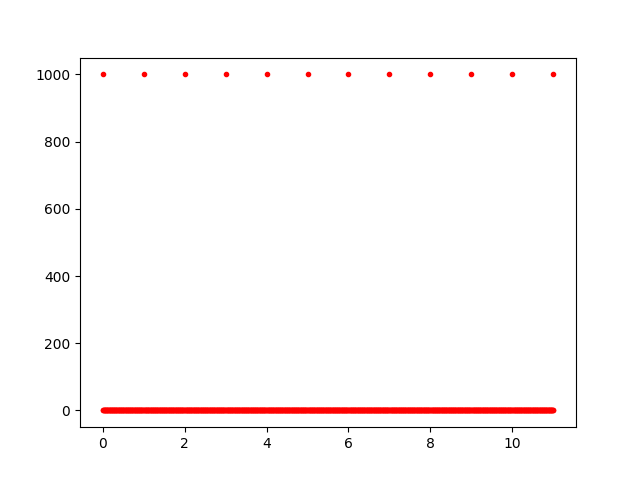
\includegraphics[width=65mm]{delta}
  \end{center}

  \captionof{figure}{Qualitative behavior of delta function potential}\label{fig:delt}\vspace{0.5cm}

  Hence, if we calculate the fourier coefficients of $U(x)$ we will have
  \begin{equation}
    \begin{aligned}[b]
      U_G &= \frac{1}{a}\int_{-a/2}^{a/2}dx U(x)e^{-iGx},\\
      &= \frac{1}{a}\int_{-a/2}^{a/2}dx \sum_s A \delta (x-sa)e^{-iGx},\\
      &= \frac{1}{a}\int_{-a/2}^{a/2}dx A \delta (x)e^{-iGx},\\
      &= \frac{A}{a}.
    \end{aligned}
  \end{equation}
To go from the second to the third line we used the fact that $s\in \mathbb{Z}$ and $\delta (x-sa)$ is non-zero just when $s=0$, for $x\in [-a/2,a/2].$ In fig. \ref{fig:four} we can see the reconstruction of the initial delta potential using the Fourier components $U_G$. AS we can see the more frequencies we add the more accurate our reconstruction is.

\begin{center}
  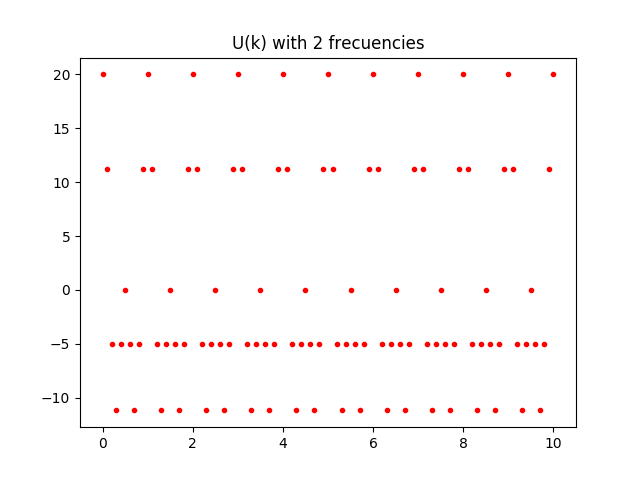
\includegraphics[width=65mm]{uk2}
  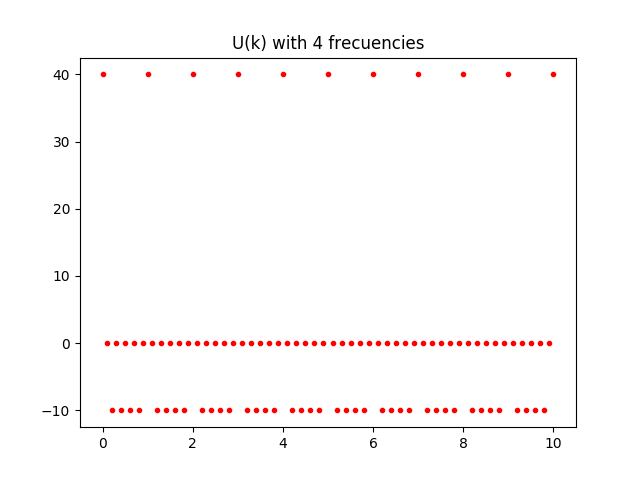
\includegraphics[width=65mm]{uk4}
  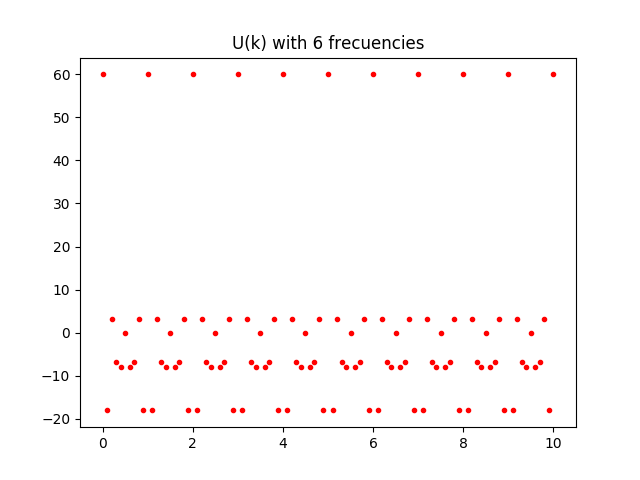
\includegraphics[width=65mm]{uk6}
  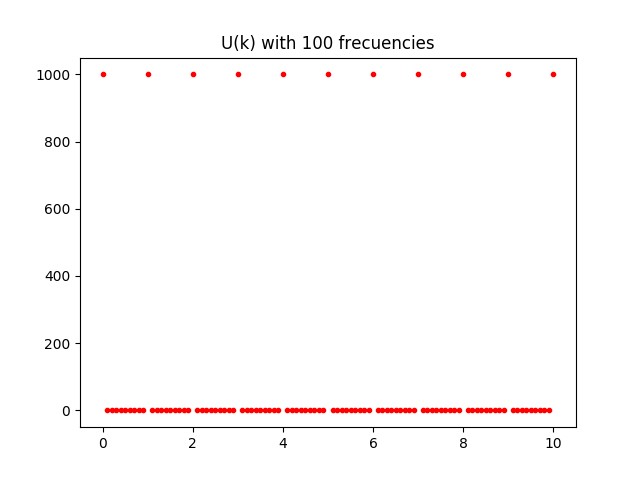
\includegraphics[width=65mm]{uk100}
\end{center}

\captionof{figure}{U(k) using 2, 4, 6, and 100 frequencies.}\label{fig:four}\vspace{0.5cm}

The final step is to actually know what is the system of equations we are going to solve numerically, for this matter we deal with the following calculations. The wave equation of an electron in a crystal is (See Kittel)

\begin{equation}
  \left(\frac{1}{2m}p^2 + \sum_G U_Ge^{iGx}\right) \psi(x) = \epsilon \psi(x).
  \label{sch}
\end{equation}

Now, assuming our solution is of the form

\begin{equation}
  \psi = \sum_k C(k)e^{ikx},
\end{equation}

and plugging this equation into eq. \ref{sch} the wave equation changes to

\begin{equation}
  \sum_k \frac{\hbar^2}{2m}k^2 C(k)e^{ikx} + \sum_G \sum_k U_GC(k)e^i{k+G}x = \epsilon \sum_k C(k)e^ikx.
\end{equation}

All Fourier components must have the same coefficient on both sides if the equation. This leads us to the central equation

\begin{equation}
  (\lambda_k -\epsilon)C(k) + \sum_G U_GC(k-G) = 0,
  \label{central}
\end{equation}
where
\begin{equation}
  \lambda_k = \frac{\hbar^2 k^2}{2m}.
\end{equation}

Solving this equation we find the following solutions (using similar parameters to the first exercise)
%
\begin{center}
  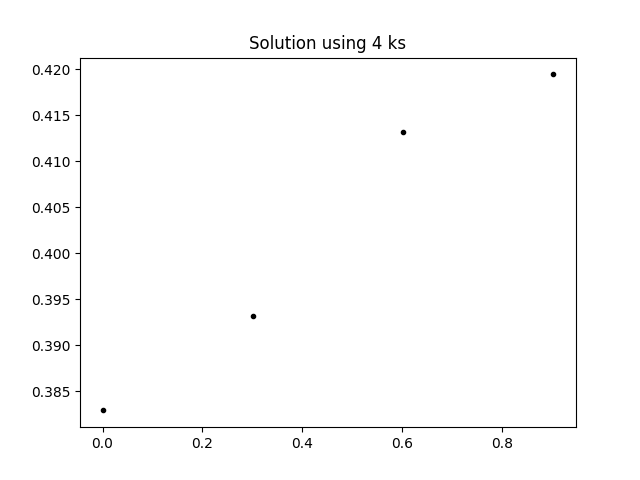
\includegraphics[width=45mm]{num4}
  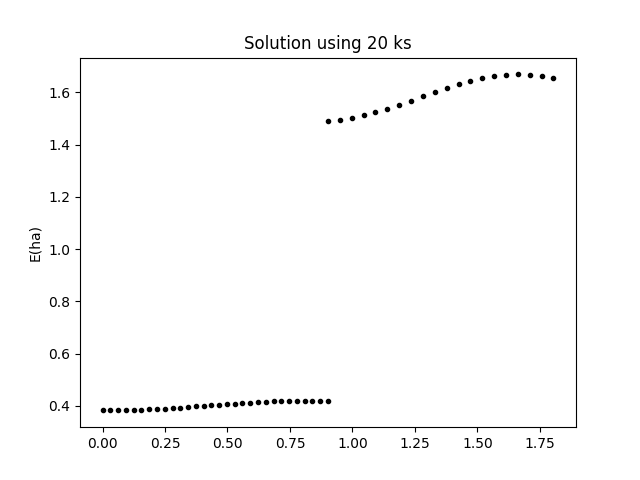
\includegraphics[width=45mm]{num20}
  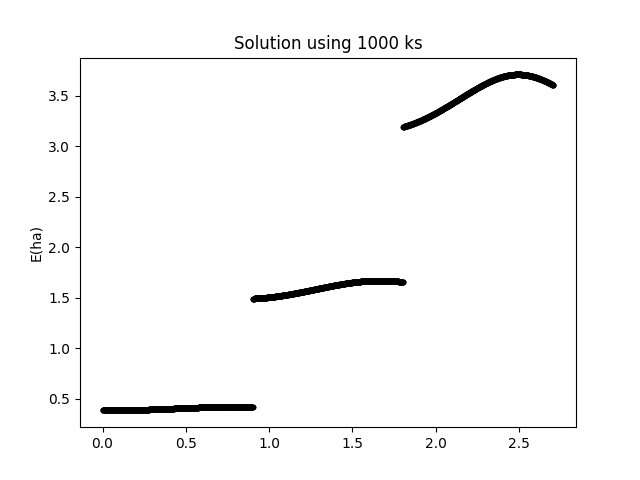
\includegraphics[width=45mm]{num1000}
\end{center}

\captionof{figure}{U(k) using 2, 4, 6, and 100 frequencies.}\label{fig:three}\vspace{0.5cm}

If we use more k values we obviously get more energies, and therefore our bands are more populated. The band-gap is determined by the lattice factors. This changes if we modify for example the lattice parameter.\\

Our solutions on this section look similar to the analytical solutions, even though we started with a delta-like potential and therefore were solving a different equation. If we pay attention that equation is actually our eq. 12. Analytically we solved eq. 11. But at the end, they yielded similar results.

 \end{solution}

\end{questions}

%
% \begin{center}
%   \includegraphics[width=55mm]{}
% \end{center}
%
% \captionof{figure}{}\label{new}\vspace{0.5cm}
